


\documentclass{notes}
\usepackage{color-env}
\usepackage[english]{babel}
\usepackage{amssymb,amsmath,amsfonts}  %%% for maths
\usepackage{bm}
%%%%%%%%%%%%%%%%%%%%%%%%%%%%%%%%%%%%%
\usepackage[object=vectorian]{pgfornament}
\usepackage{background}
\usepackage{calligra}
\usepackage{enumerate} %% it make lists
%\usepackage{semantic} 
%\usepackage{graphicx} %%% \to include figures 
%\usepackage{subfig} %%%% for two figures side by side
\renewcommand\qedsymbol{$\blacksquare$}
%%%%%%%%%%%%%%%%%%%%%%%%%%%%%%%%%%%%%
%%%%%%%%%%%%%%%%%%%%%%%%%%%%%%%%%%%%
\newcommand{\norm}[1]{\left\lVert #1 \right \rVert} 
\newcommand{\abs}[1]{\left| #1 \right|}
\newcommand{\bgamma}{\bm{\gamma}}
\newcommand{\R}[1]{\mathbb{R}^{#1} }
\newcommand{\bsigma}{\bm{\sigma}}


\begin{document}

	\begin{titlepage} % Suppresses headers and footers on the title page
		\backgroundsetup{
			scale=1,
			opacity=1,
			angle=0,
			color=black,
			contents={
			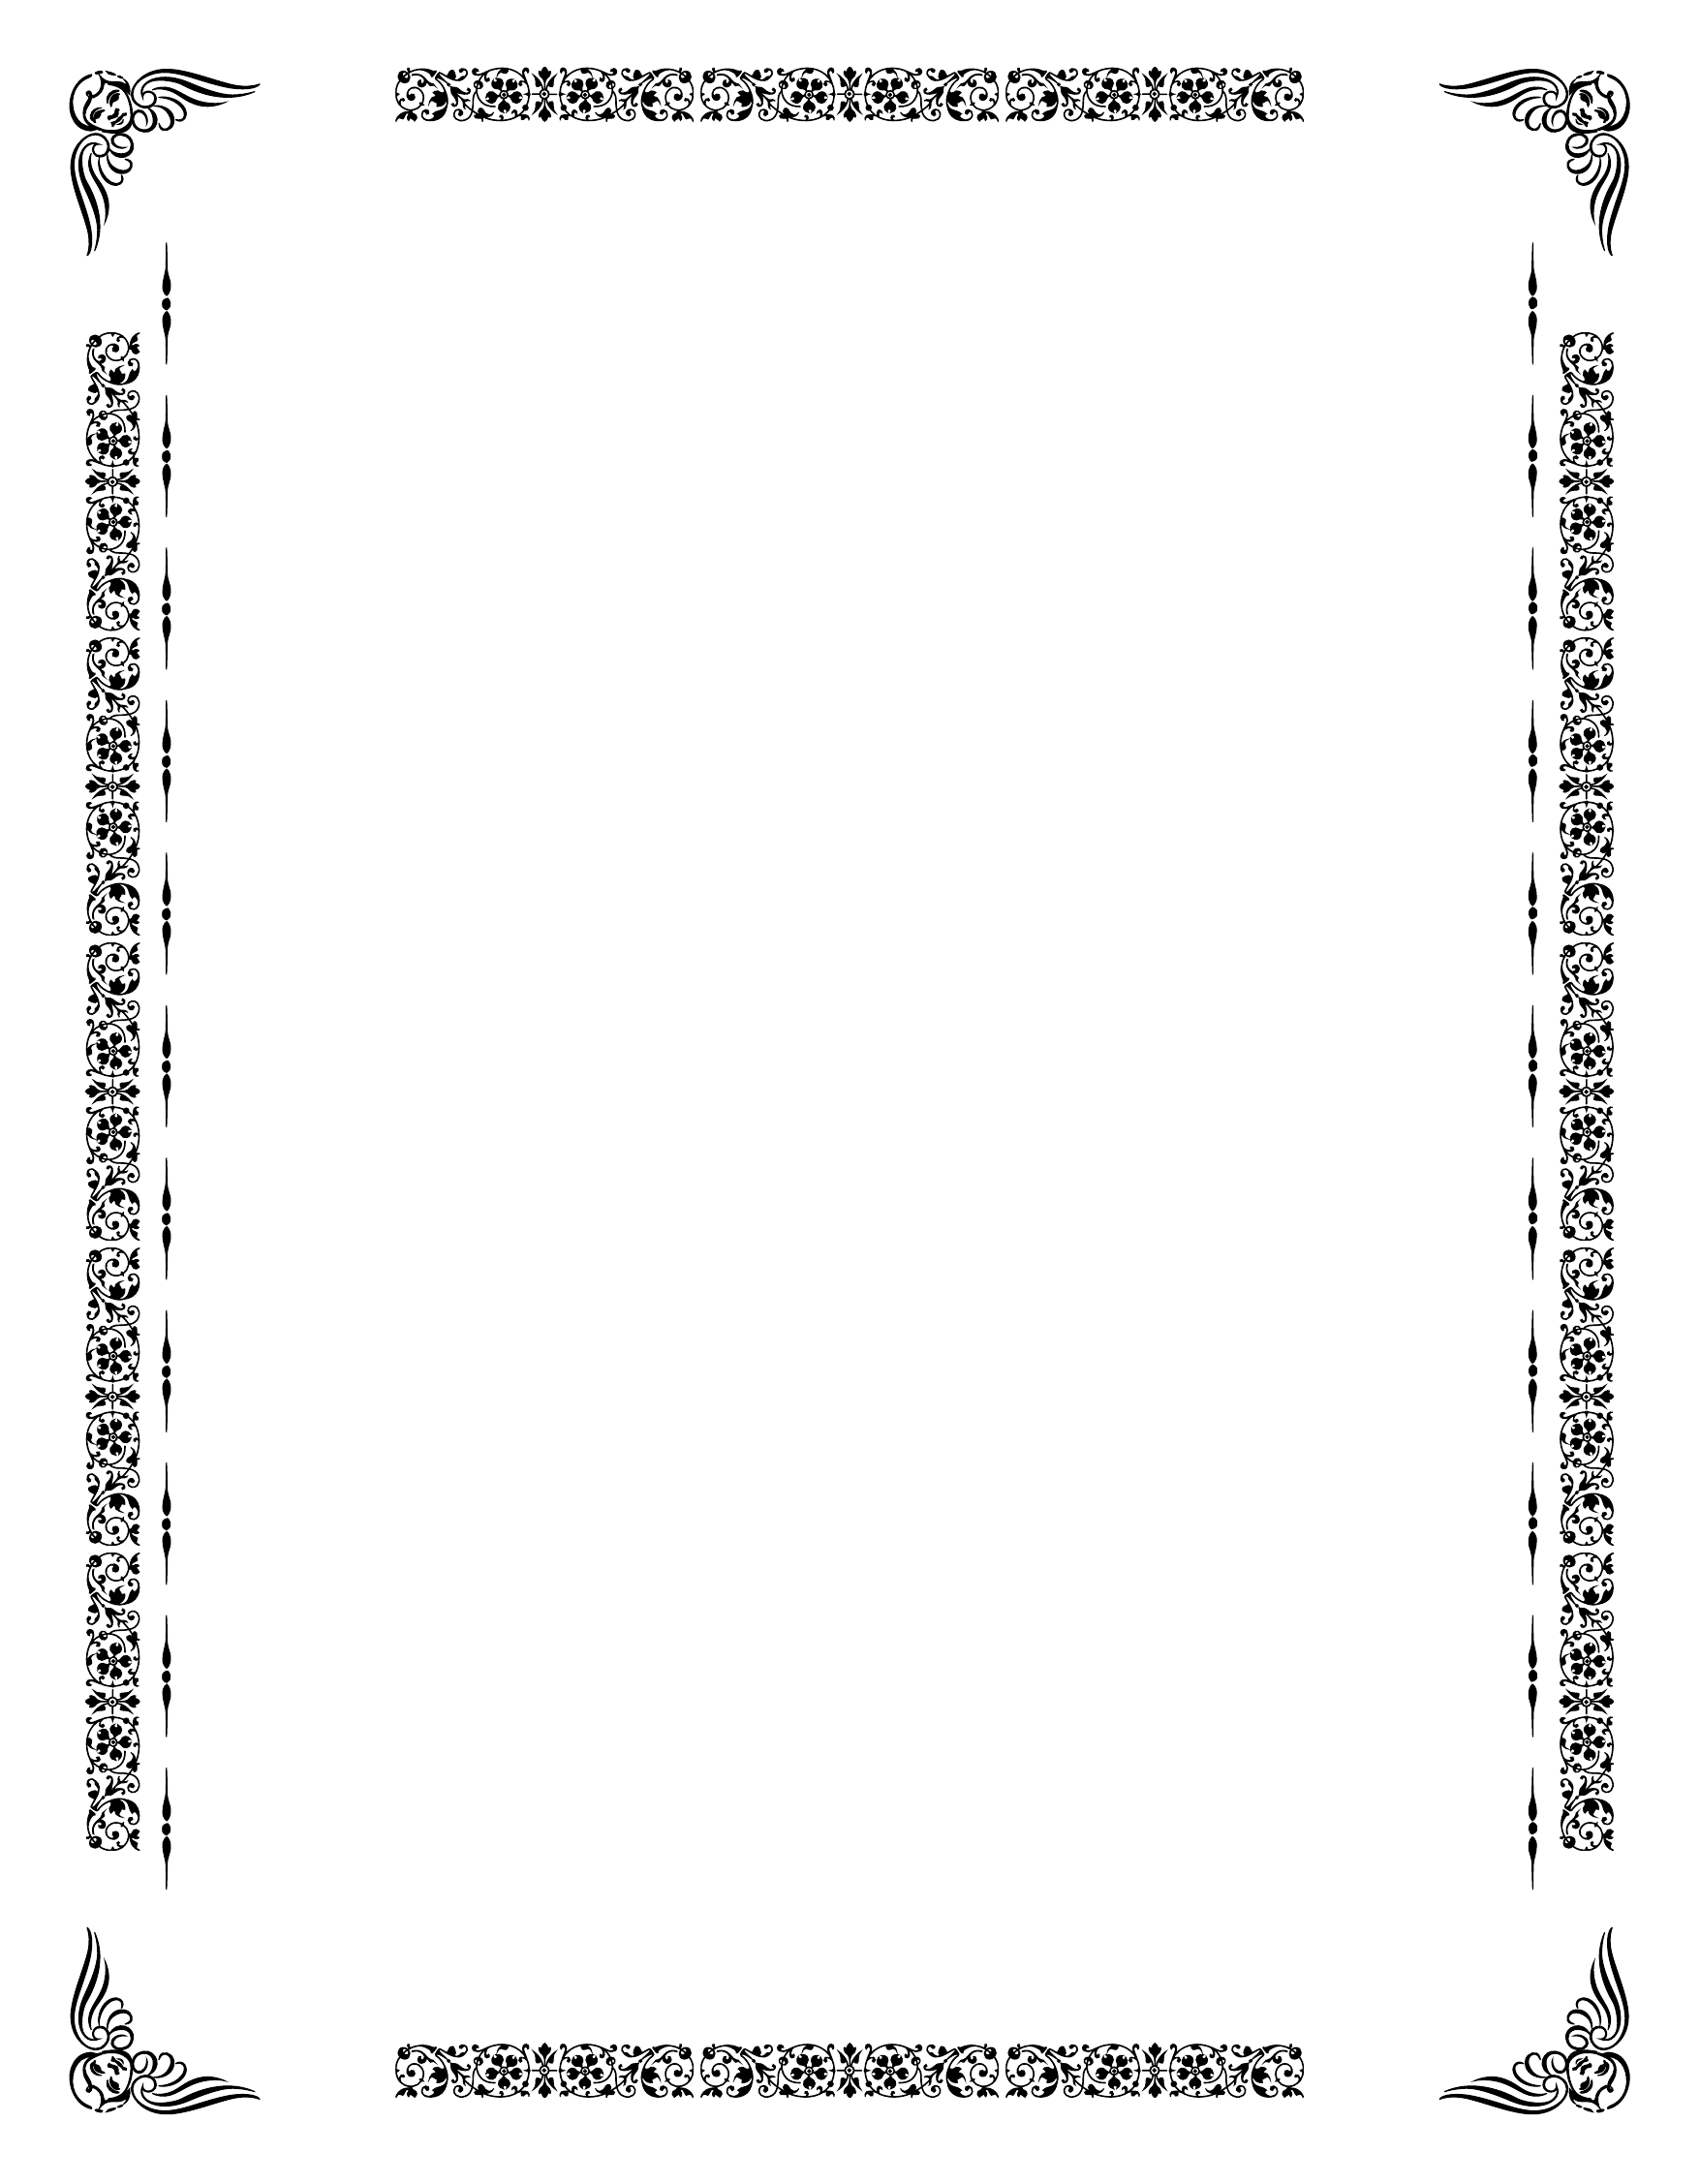
\begin{tikzpicture}[color=black, every node/.style={inner sep= 15pt}]
				\node (NW) [anchor=north west] at (current page.north west){\pgfornament[width=2.5cm] {131}};
				\node (NE) [anchor=north east] at (current page.north east){\pgfornament[width=2.5cm, symmetry=v]{131}};
				\node (SW) [anchor=south west] at (current page.south west){\pgfornament[width=2.5cm, symmetry=h]{131}};
				\node (SE) [anchor=south east] at (current page.south east){\pgfornament[width=2.5cm, symmetry=c]{131}};
				\foreach \i in {-4,0,4}
				\node[anchor=north,xshift=\i cm] at (current page.north){\pgfornament[scale=0.25,symmetry=v]{71}};
				\foreach \i in {-4,0,4}
				\node[xshift=\i cm, yshift=32.25 pt] at (current page.south){\pgfornament[scale=0.25,symmetry=v]{71}};
				\foreach \i in {-8,-4,0,4,8}
				\node[yshift=\i cm, xshift=32.25pt, rotate=90] at (current page.west){\pgfornament[scale=0.25,symmetry=v]{71}};
				\foreach \i in {-8,-4,0,4,8}
				\node[yshift=\i cm, xshift=-32.25pt, rotate=90] at (current page.east){\pgfornament[scale=0.25,symmetry=v]{71}};
				\foreach \i in {-11,-9,...,7,9}
				\node[anchor=west, yshift=\i cm, xshift=52.25pt, rotate=90] at (current page.west){\pgfornament[scale=0.1]{80}};
				\foreach \i in {-11,-9,...,7,9}
				\node[anchor=east, yshift=\i cm, xshift=-52.25pt, rotate=-90] at (current page.east){\pgfornament[scale=0.1]{80}};
			\end{tikzpicture}
}}
		
		\centering % Centre everything on the title page
		
		\scshape % Use small caps for all text on the title page
		
		\vspace*{\baselineskip} % White space at the top of the page
		
		%------------------------------------------------
		%	Title
		%------------------------------------------------
		
		\rule{\textwidth}{1.6pt}\vspace*{-\baselineskip}\vspace*{2pt} % Thick horizontal rule
		\rule{\textwidth}{0.4pt} % Thin horizontal rule
		
		\vspace{0.75\baselineskip} % Whitespace above the title
		
		{\huge \calligra{Differential Geometry}\\} % Title
		
		\vspace{0.75\baselineskip} % Whitespace below the title
		
		\rule{\textwidth}{0.4pt}\vspace*{-\baselineskip}\vspace{3.2pt} % Thin horizontal rule
		\rule{\textwidth}{1.6pt} % Thick horizontal rule
		
		\vspace{2\baselineskip} % Whitespace after the title block
		
		%------------------------------------------------
		%	Subtitle
		%------------------------------------------------
		
		\LARGE{MTH201} 
		
		\vspace*{3\baselineskip} % Whitespace under the subtitle
		
		%------------------------------------------------
		%	Editor(s)
		%------------------------------------------------
		
		
		\vspace{0.5\baselineskip} % Whitespace before the editors
		
		%{\scshape   \LARGE Prof. Vaibhav Vaish\\ } % Editor list
		
		\vspace{0.5\baselineskip} % Whitespace below the editor list
		
		%\textit{\Large IISER, Mohali} % affiliation
		
		\vfill % Whitespace between editor names and publisher logo
		
		%------------------------------------------------
		% Author
		%------------------------------------------------
		
		
		\vspace{0.3\baselineskip} % Whitespace under the publisher logo
		
		
		{\large Edited by\\  Aditya Dev} 
		
	\end{titlepage}
	\backgroundsetup{contents={}} 
	\tableofcontents
%\newpage
\chapter{Curves in the plane and in space}

\section{What is a curve?}

\begin{definition}[Parametrized curve]{def:curve}
	A \textit{parametrized curve} in \(\mathbb{R}^n\) is a map \(\bm{\gamma}: (\alpha, \beta) \to \mathbb{R}^n\), for some \((\alpha, \beta) \subseteq \mathbb{R}\)
	
\paragraph{Example}: \(\bm{\gamma}(t): (-\infty, \infty) \to (t, t^2)\)
\end{definition}

\begin{description}
	\item[Note] There can be different parametrizations for the same curve; but it's not mandatory that they have same properties.
	\item[Smooth Function] 
	 A function \(f: (\alpha, \beta) \to \mathbb{R}\) is said to be
	smooth if the derivative \(\frac{d^n f}{dt^n}\) exists for all $n \geq 1$ and all $t \in (\alpha, \beta)$.
\end{description}
\begin{definition}[Tangent Vector]{def:tangent}
	If \(\bm{\gamma}\) is a parametrized curve, its first derivative \(\dot{\bm{\gamma}}(t)\) is called the tangent vector
	of \(\bm{\gamma}\) at the point \(\bm{\gamma}\)$(t)$.
\end{definition}

\begin{proposition}{prop:staright-line}
	If the tangent vector of a parametrized curve is constant, the image of the curve
	is (part of) a straight line.
\end{proposition}


\section{Arc-Length}
\paragraph{Recall that} if \(\mathbf{v} = (v_1, v_2, \ldots v_n) \in \mathbb{R}^n\), then it's length is:
\[ \norm{\mathbf{v}} = \sqrt{v_1 ^2 + v_2 ^2 + \cdots v_n ^2}\] 
If \(\mathbf{u}\) is another vector in \(\mathbb{R}^n\) , \(\norm{\mathbf{u} - \mathbf{v}}\) is the length of the straight line segment joining the points \(\mathbf{u}\) and \(\mathbf{v}\) in \(\mathbb{R}^n\).

\begin{definition}[Arc-length]{def:arc-length}
	The \textit{arc-length} of a curve \(\bm{\gamma}\) starting at the point \(\bm{\gamma}(t_0)\) is the function \(s(t)\) given by:
	\[s(t) = \int_{t_0}^{t} \norm{\dot{\bm{\gamma}}(x)} dx\]
	
	Note that if we choose a different starting point, then the new arc-length differs from the previous one (\textit{but how much?})
\end{definition}

\begin{definition}{def:unit-speed}
	If \(\bm{\gamma}: (\alpha, \beta) \to \mathbb{R}^2\) is a parametrized curve, it's speed at point \(\mathbf{\bm{\gamma}}(t)\) is \(\norm{\dot{\bm{\gamma}}(t)}\), and \(\bm{\gamma}\) is said to be a unit-speed curve if \(\dot{\bm{\gamma}}(t)\) is a unit-vector \(\forall t\in (\alpha, \beta)\).
\end{definition}

\begin{proposition}{prop:unit-zero}
	Let \(\mathbf{n}(t)\) be a unit vector that is a smooth function of a parameter \(t\). Then, the dot product
	\[\mathbf{n}(t) \cdot \dot{\mathbf{n}}(t) = 0 \quad \forall t\]
	so, either \(\dot{\mathbf{n}}(t)\) is zero or perpendicular to \({\mathbf{n}}(t)\)

\end{proposition}

\section{Reparametrization of a curve}

\begin{definition}[Reparametrization]{def:repar}
A parametrized curve \(\tilde{\bm{\gamma}}: (\tilde{\alpha}, \tilde{\beta}) \to \mathbb{R}^n\) is a reparametrization of a parametrized curve \(\bm{\gamma}: (\alpha, \beta) \to \mathbb{R}^n\) if \(\exists\) a smooth bijective map \(\phi: (\tilde{\alpha}, \tilde{\beta}) \to (\alpha, \beta)\) (the reparametrization map) such that the inverse map \(\phi^{-1}: (\alpha, \beta) \to (\tilde{\alpha}, \tilde{\beta})\) is also smooth and
\[\tilde{\bm{\gamma}}(\tilde{t}) = \bm{\gamma}(\phi(\tilde{t}))\]
\end{definition}

\begin{definition}[Regular Curve]{:def:regular-curve}
	A point \(\bm{\gamma}(t)\) of a parametrized curve \(\bm{\gamma}\) is called a regular point if \(\dot{\bm{\gamma}}(t) \not = 0\)
	otherwise \(\bm{\gamma}(t)\) is a singular point of \(\bm{\gamma}\). A curve is regular if all of its points are regular
\end{definition}

\begin{proposition}{}
	Any reparametrization of a regular curve is regular.
\end{proposition}
\begin{proposition}{prop:1.3.2}
	If \(\bm{\gamma}(t)\) is a regular curve, its arc-length \(s\), starting at any point of \(\bm{\gamma}\), is smooth function of \(t\).
\end{proposition}


\begin{theorem}[Unit-speed reparametrization]{def:unit-repar}
	A parametrized curve has a unit-speed reparametrization if and only if it is
	regular.
\end{theorem}
\begin{corollary}{1}
	Let \(\bm{\gamma}\) be a regular curve and let \(\tilde{\bm{\gamma}}\) be a unit-speed reparametrization of \(\bm{\gamma}\):
	\[\tilde{\bm{\gamma}}(u(t)) = \bm{\gamma}(t) \quad \forall t\]
	where \(u\) is a smooth function of \(t\). Then, if \(s\) is the arc-length of \(\bm{\gamma}\) (starting at any point), we have:
	\[u = \pm s + c \quad \text{for some } c \in \mathbb{R} \tag*{(1.1)}\]
	Conversely, if \(u\) is given by Eq. \(1.1\) for some value of \(c\)
	and with either sign, then \(\tilde{\bm{\gamma}}\) is a unit-speed reparametrization of \(\bm{\gamma}\).
\end{corollary}
\section{Closed Curves}

\begin{definition}[Periodic Curve]{def:periodic}
	Let \(\bm{\gamma}: \mathbb{R} \to \mathbb{R}^n\) be a smooth curve and let \(T \in \mathbb{R}\). We say that \(\bm{\gamma}\) is
	\(T\) -periodic if:
	\[\bm{\gamma}(t +T) = \bm{\gamma}(t) \quad \forall t\in \mathbb{R}\]
	If \(\bm{\gamma}\) is not constant and is \(T\)-periodic for some \(T \not = 0\), then \(\bm{\gamma}\) is said to be closed.
	
	\textbf{Note} if \(\bm{\gamma}\) is \(T\)-periodic the it is \(-T\)-periodic too because
	\[\bm{\gamma}(t - T) = \bm{\gamma}(t -T + T) = \bm{\gamma}(t)\]
	It follows that if \(\bm{\gamma}\) is \(T\)-periodic for some \(T \not = 0\), then it is \(T\)-periodic for some
	$(T > 0)$.
\end{definition}

\begin{definition}[Self-intersection]{def:self-intersection}
	A curve \(\bm{\gamma}\) is said to have a self-intersection at a point \(\mathbf{p}\) of the curve if there
	exist parameter values \(a \not = b\) such that
	\begin{itemize}
		\item \(\bm{\gamma}(a) =\bm{\gamma}(b) = \mathbf{p} \)
		\item if \(\bm{\gamma}\) is closed with period \(T\) , then \(a - b\) is not an integer multiple of \(T\) .
	\end{itemize}
\end{definition}

\begin{proof}
	Assume there exists no lower bond for the period of curve. 
	Then if \(T_1\) is the period of \(\bgamma\) then \(\exists\  T_2\) such that \(T_2\) is also the period of the curve and by iteration we can show:
	\[T_1 > T_2 > T_3 \ldots >0\]
	is a sequence of the periods for curve \(\bgamma\)
	
Since, the sequence is bounded and monotonic, therefore \(\lim\limits_{r \to \infty} T_r = T\) i.e the sequence is convergent \(\implies\) the sequence is cauchy.

And by definition of cauchy sequence:
\[\forall \epsilon > 0\ \exists N : \forall m, n> N \implies \abs{T_m -T_n} < \epsilon\]

Let, \(T_m > T_n\) (won't change the definition).Also, we know that if \(T_m \ \& \ T_n\) are periods of \(\bgamma\) \(\implies T_m - T_n \implies T_m = T_n + \epsilon\)  is also the period of gamma (trivial to prove!). 
\[
\begin{gathered}
	\bgamma(t + T_n + \epsilon) = \bgamma(t) \\
	\bgamma(t + \epsilon) = \bgamma(t)
\end{gathered}
\]

Since, it's true \(\forall \epsilon > 0 \implies \bgamma\) is constant. 
%\[\implies \dfrac{d \bgamma}{dt} =\lim\limits_{\epsilon \to 0} \dfrac{\bgamma(t + \epsilon) - \bgamma(t)}{\epsilon}  = 0 \]
Hence, a contradiction (\(\bgamma\) is non-constant.). So, our assumption was false.
\end{proof}

\chapter{Curvature}

\section{What is curvature?}
\begin{definition}[Curvature]{def:curvature}
	If \(\bm{\gamma}\) is a unit-speed curve with parameter \(t\), its curvature \(\kappa(t)\) at the point \(\bm{\gamma}(t)\)
	is defined to be \(\norm{\ddot{\bm{\gamma}}(t)}\).
	
\textbf{Note} we have defined curvature for a unit-speed parametric ony.
\end{definition}
\begin{theorem}{1}
	The curvature for any regular curve \(\bm{\gamma}\) is given as
	\[\kappa = \dfrac{\norm{ (\dot{\bm{\gamma}}\cdot\dot{\bm{\gamma}}) \ddot{\bm{\gamma}} - (\dot{\bm{\gamma}}\cdot\ddot{\bm{\gamma}}) \dot{\bm{\gamma}}}}{\norm{\dot{\bm{\gamma}}}^4} \]
 \end{theorem}
\begin{proposition}{1}
	Let \(\bm{\gamma}(t)\) be a regular curve in \(\mathbb{R}^3\). Then its curvature is 
	\[\kappa = \dfrac{\norm{\ddot{\bm{\gamma}} \times \dot{\bm{\gamma}}}}{\norm{\dot{\bm{\gamma}}}^3}\]
	where \(\times\) is our usual vector cross product.
\end{proposition}

\begin{problem}
	Show that, if the curvature \(\kappa(t)\) of a regular curve \(\bm{\gamma}(t) \) is \(>0\) every-
	where, then \(\kappa(t)\) is a smooth function of \(t\). Give an example to show
	that this may not be the case without the assumption that \(\kappa(t >0)\).
\end{problem}

\section{2D and 3D curves}
\subsection{Plane curve}
Let \(\bm{\gamma}\) be a unit-speed curve in a plane. And let the tangent vector be
\[\mathbf{t} = \dot{\bm{\gamma}}\]
Note, \(\mathbf{t}\) is a unit-vector. There are two vectors perpendicular to \(\mathbf{t}\);  we make a choice by defining \(\mathbf{n}_s\), the \textit{signed unit normal} of \(\bm{\gamma}\), to be the unit vector obtained by rotating \(\mathbf{t}\) anti-clockwise by \(\pi/2 \)

So, by Proposition \ref{prop:unit-zero}, \(\dot{\mathbf{t}} = \ddot{\bm{\gamma}}\) is perpendicular to \(\mathbf{t}\), and hence parallel to \(\mathbf{n}_s\). Thus, there is a scalar \(\kappa_s\) such that
\[\ddot{\bm{\gamma}}= \kappa_s \mathbf{n}_s\]
\(\kappa_s\) is called the signed curvature of \(\bm{\gamma}\). And since \(\norm{\mathbf{n}_s} = 1\), we have
\[\kappa = \norm{\kappa_s \mathbf{n}_s} = \abs{\kappa_s}\]

Note, we have defined the signed curvature for unit-speed curve. If \(\bm{\gamma}\) is any regular curve , the we define the above defined parameters to be those of it's unit speed parametrization. 


Intuitively, since \(\bm{\gamma}(t)\) is assumed to be a unit-speed curve on a plane, then \(\dot{\bm{\gamma}}(t)\) can be measured by angle \(\phi(s)\) such that:
\[\dot{\bm{\gamma}}(s) = (\cos \phi (s), \sin \phi(s)) \tag*{(2)}\]
Also, we can think curvature as rate at which the angle of tangent vector is changing, so if we find the derivative of the above curve then it simply represents a changing angle parameter. 

\begin{proposition}{prop:gg}
	Let \(\bm{\gamma}: (\alpha, \beta) \to \mathbb{R}^2\) be a unit speed curve, let \(s_0 \in (\alpha, \beta)\) and let \(\phi _0 \) be such that 
	\[\dot{\bm{\gamma}}(s_0) = (\cos \phi _0, \sin \phi_0) \]
	Then \(\exists!\) smooth function: \(\phi: (\alpha, \beta) \to \mathbb{R}\) such that \(\phi(s_0) = \phi _ 0\) and that Eq. (2) holds for all \(s \in (\alpha, \beta)\)
\end{proposition}

\begin{definition}[Turning Angle]{def:turning-angle}
The smooth function \(\phi\) in Proposition \ref{prop:gg} is called the turning angle of \(\bm{\gamma}\)
determined by the condition \(\phi(s_0) = \phi_0\) .
\end{definition}

\begin{proposition}{def:intut-signed-curvature}
Let \(\bm{\gamma}(s)\) be a unit-speed plane curve, and let \(\phi(s)\) be a turning angle for \(\bm{\gamma}\).
Then,
\[\kappa _s = \dfrac{d\phi}{ds}\]
Thus, \textbf{the signed curvature is the rate at which the tangent vector of the
curve} rotates.
\end{proposition}

\begin{corollary}{}
	The total signed curvature of a closed plane curve is an integer multiple of \(2\pi\)
\end{corollary}
\par 

The next result shows that a unit-speed plane curve is essentially determined
once we know its signed curvature at each point of the curve. The meaning of
`essentially’ here is `up to a direct isometry of \(\mathbb{R}^2\) ’, i.e., a map \(M: \mathbb{R}^2 \to \mathbb{R}^2\) of
the form
\[M  = T_a \circ \rho_\theta\]
where \(\rho _\theta\) is an anti-clockwise rotation by angle \(\theta\) about the origin,
\[\rho _\theta  = (x\cos \theta - y \sin \theta, x \sin \theta + y \cos \theta)\]
and \(T_a\) is a translation by vector \textbf{a}
\[T_a (\mathbf{v}) = \mathbf{v}+ \mathbf{a}\]
for any vector \((x, y) \) and \(\mathbf{v}\) in \(\mathbb{R}^2\)


\begin{theorem}{theo:1}
	Let \(k : (\alpha, \beta) \to \mathbb{R}\) be any smooth function. Then, there is a unit-speed curve
	 \(\bm{\gamma}:(\alpha, \beta)\to \mathbb{R}^2\) whose signed curvature is  k.
	
	Further, if \(\tilde{\bm{\gamma}}: (\alpha, \beta)\to \mathbb{R}^2\) is any other unit-speed curve 
	whose signed curvature is \(k\), there is a direct isometry \(M\) of \(\mathbb{R}^2\) such that
	\[\tilde{\bm{\gamma}}(s) = M(\bm{\gamma}(s)) \ \forall s \in (\alpha, \beta) \]
\end{theorem}

\subsection{Space curve}

\begin{definition}{def:princ-normal}
	Let \(\bm{\gamma}(s)\) be a unit-speed curve in \(\mathbb{R}^3\) , and let \(\mathbf{t} = \dot{\bm{\gamma}}\) be its unit tangent
	vector. If the curvature \(\kappa_s\) is non-zero, we define the principal normal of \(\bm{\gamma}\)
	at the point \(\bm{\gamma}(s)\) to be the vector
\[\mathbf{n}(s) = \frac{1}{\kappa(s)} \mathbf{\dot{t}}(s)\]
Further, since \(\lVert\mathbf{\dot{t}}\rVert = \kappa\), so \(\mathbf{n}\) is a unit-vector. Therefore by Proposition 
\ref{prop:unit-zero}, so \(\mathbf{t}\) and \(\mathbf{n}\) are perpendicular.So
\[\mathbf{b} = \mathbf{t} \times \mathbf{n}\]
is a unit-vector perpendicular to both \(\mathbf{t}\) and \(\mathbf{n}\). The vector \(\mathbf{b}(s)\) is called the 
\textit{binormal} vector of \(\bm{\gamma}\) at point \(\bm{\gamma}(s)\). Thus, \(\{ \mathbf{t}, \mathbf{n}, \mathbf{b}\}\) is an
 orthonormal basis of \(\mathbb{R}^3\)
, and is \textit{right-handed}.
\end{definition}

\begin{definition}{def:torison}
	From Definition \ref{def:princ-normal} we have
	\[\mathbf{b} = \mathbf{t} \times \mathbf{n}\]
	Differentiating both sides gives
	\[\dot{\mathbf{b}} = \dot{\mathbf{t}} \times \mathbf{n} + \mathbf{t} \times \dot{\mathbf{n}} = \mathbf{t} \times \dot{\mathbf{n}} \tag{(3)}\]
	Equation (3) shows
	that \(\dot{\mathbf{b}}\) is perpendicular to \(t\). Being perpendicular to both \(\mathbf{t}\) and \(\mathbf{b}\), \(\dot{\mathbf{b}}\) must be
	parallel to \(\mathbf{n}\), so
	\[\dot{\mathbf{b}} = -\tau \times  \mathbf{n}\]
	for some scalar \(\tau\) , which is called the \textit{torsion} of \(\bm{\gamma}\).
	
	\textbf{Note} that the torsion
	is only defined if the curvature is non-zero.
\end{definition}

\begin{definition}{prop:torison}
	Let \(\bm{\gamma}(t)\) be a regular curve in \(\mathbb{R}^3\) with nowhere-vanishing curvature. Then,
	denoting \(\frac{d}{dt}\) by a dot, its torsion is given by
	\[\tau = \dfrac{(\dot{\bm{\gamma}} \times \ddot{\bm{\gamma}})\cdot\dddot{\bm{\gamma}}}{\norm{\dot{\bm{\gamma}} \times \ddot{\bm{\gamma}}}^2}\]
\end{definition}

\begin{proposition}{1}
	Let \(\bm{\gamma}\)  be a regular curve in \(\mathbb{R}\) with nowhere vanishing curvature (so that the
	torsion \(\tau\) of \(\bm{\gamma}\) is defined). Then, the image of \(\bm{\gamma}\) is contained in a plane if and
	only if \(\tau\) is zero at every point of the curve.
\end{proposition}
\begin{theorem}{theo:frenet-serret}
	
	Let \(\bm{\gamma}\) be a unit-speed curve in \(\mathbb{R}\) with nowhere vainshing curvature. Then, 
	\[
	\begin{gathered}
		\mathbf{\dot{t}} = \kappa \mathbf{n}\\
		\mathbf{\dot{n}} = -\kappa \mathbf{t} + \tau \mathbf{b}\\
		\mathbf{\dot{b}} = \tau \mathbf{n}
	\end{gathered}
	\]
	
	The above equation is called as \textit{Frenet-Serret equations}. Notice that the matrix
	\[
	\left(
	\begin{array}{c c c}
		0 & \kappa & 0 \\
		-\kappa & 0 & \tau\\
		0 & -\tau & 0 
	\end{array}
	\right)
	\]
	which is the matrix of linear transformation is a \textit{skew-symmetric}.
\end{theorem}

\begin{proposition}{1}
	Let \(\bm{\gamma}\) be a unit-speed curve in \(\mathbb{R}^3\) with constant curvature and zero torsion.
	Then, \(\bm{\gamma}\) is a parametrization of (part of) a circle.
\end{proposition}

\begin{theorem}{1}
	Let \(\bm{\gamma}(s)\) and \(\tilde{\bm{\gamma}}(s)\) be two unit-speed curves in \(\mathbb{R}^3\) with the same curvature
	\(\kappa(s) >0 \) and the same torsion \(\tau(s)\) for all \(s\). Then, there is a direct isometry
	\(M\) of \(\mathbb{R}^3\) such that
\[\tilde{\bm{\gamma}}(s) = M(\bm{\gamma}(s)) \quad \forall s\]
	Further, if \(k\) and \(t\) are smooth functions with \(k > 0\) everywhere, there is a
	unit-speed curve in \(\mathbb{R}^3\) whose curvature is \(k\) and whose torsion is \(t\).
\end{theorem}

\chapter{Global properties of curves}

\section{Simple closed curves}

\begin{definition}{def:closed-curves}
	A \textit{simple closed curve} in \(\mathbb{R}^2\) is a closed curve in \(\mathbb{R}^2\) that has no self-intersections.
\end{definition}

\begin{theorem}[Jordan Curve Theorem]{thm:jordan-curve-theorem}
The complement of the image of \(\bgamma\)
(i.e., the set of points of \(\mathbb{R}^2\) that are not in the image of $\bgamma$) is the disjoint
union of two subsets of \(\mathbb{R}^2\), denoted by \(\mathrm{int}( \bgamma)\) and \(\mathrm{ext}(\bgamma)\), with the following
properties:

\begin{itemize}
	\item \(\mathrm{int}(\bgamma)\) is bounded, i.e. it is contained in the circle of sufficiently large radius.
	\item \(\mathrm{ext}(\bgamma)\) is unbounded.
	\item Both the regions \(\mathrm{int}(\bgamma)\) and \(\mathrm{ext}(\bgamma)\) are connected, i.e they have the property that any two points in the same region can be joined by a curve contained entirely in the region. 
\end{itemize}

\end{theorem}

\begin{theorem}[Hopf’s Umlaufsatz]{def:Hopf-Umlaufsatz}
The total signed curvature of a simple closed curve in \(\mathbb{R}^2\) is \(\pm 2\pi\).
\end{theorem}


\section{The isoperimetric inequality}


\begin{definition}[Area of a curve]{}
	The area contained by a simple closed curve \(\bgamma\) is
	
\[\mathcal{A}(\bgamma) =\int_{\mathrm{int}(\bgamma)} dx dy\]

\end{definition}

\begin{theorem}[Green's Theorem]{thm:green-func}
\textit{Let $f (x, y)$ and $g(x, y)$ be smooth functions (i.e., functions
	with continuous partial derivatives of all orders), and let \(\bgamma\) be a positively-
	oriented simple closed curve. Then,}
\[\int_{\mathrm{int}(\bgamma)} \left(\dfrac{\partial g}{\partial x} -\dfrac{\partial f}{\partial y} \right)dxdy = \int_{\bgamma} f(x, y) dx + g(x, y)dy\]
\end{theorem}

\begin{proposition}{}
	If \(\bgamma(t) = (x(t), y(t))\) is a positively-oriented simple closed curve in \(\mathbb{R}^2\) with 
	period \(T\), then 
	\[\mathcal{A}(\bgamma) = \frac{1}{2} \int_{0}^{T} (x \dot{y} - y \dot{x}) dt\]
\end{proposition}

\begin{theorem}[Isoperimetric Inequality]{}
	Let \(\bgamma\) be a simple closed curve, let \(l(\bgamma)\) be its length and let \(\mathcal{A}(\bgamma)\) be the area
	contained by it. Then,
	\[\mathcal{A}(\bgamma) \leq \frac{1}{4\pi} l(\bgamma) ^2\]
	and equality holds if and only if \(\bgamma\) is a circle.
\end{theorem}
\section{The four vertex Theorem}

\begin{definition}[Vertex]{}
	A \textit{vertex }of a curve \(\bgamma(t)\) in \(\mathbb{R}^2\) is a point where its signed curvature \(\kappa_s\) has a stationary point, i.e., where 
	\(\frac{d \kappa_s}{d t} = 0\).
\end{definition}

\begin{theorem}[Four Vertex Theorem]{}
	Every convex simple closed curve in \(\mathbb{R}^2\) has at least four vertices.
\end{theorem}


\chapter{3D Surfaces}
\section{What is a surface?}
\paragraph{}
As in the case of curves, we make two definitions of the concept of surface. One of them (regular
surface) emphasizes the fact that a surface, as we think of it, is a set of points.
The other (parametrised surface) emphasizes the parametrization of the surface. While these two concepts
were similar in the case of curves (every regular curve can be covered with a single parametrization,
so it is a parametrised regular curve), they are different for surfaces: a sphere, for example, is a
regular surface, but not a parametrised regular surface. We will further show that we need two parametric maps
to describe the whole surface of a sphere and to keep it consistent with the other properties such as tangents amd normals etc.


\begin{definition}[Surface]{def:surface}
	A subset \(S\) of \(\mathbb{R}^3\) is a surface if, for every point \(\mathbf{p} \in S\), there is an open set \(U
	\subseteq \mathbb{R}^2\)
    and an open set \(W \subseteq \mathbb{R}^3\) containing \(\mathbf{p}\) such that \(S\cap W\) is homeomorphic
	to \(U\) i.e.
	\[\bsigma: U\subset \R{2} \to S\cap W \]
	such that \(\exists \ (u, v) \in U : \bsigma(u, v) = \mathbf{p}\).
	\end{definition}
	\begin{description}
		\item[1] A subset of \(S\) of the form \(S\cap W\), where \(W\) is an open subset
		of \(\mathbb{R}^3\) , is called an open subset of \(S\). 
		\item[2] A continuous bijective function between two topological space (i.e. shapes here) is termed
		as \textit{homeomorphism}
	\end{description}

\begin{definition}[Surface Patch]{def:patch}
	A homeomorphism \(\bsigma : U \to S \cap W\) as in
	previous definition is called a \textit{surface patch or parametrization} of the open subset
	\(S\cap W\) of \(S\).
\end{definition}
\begin{description}
	\item[] A surface is some subset of R3
	that can be covered by surface patches. Each surface patch looks like a (maybe deformed) piece
	of \(\R{2}\).
\end{description}

 
\section{Smooth Surfaces}
 \begin{description}
	 \item[Smooth Functions] If \(U\) is an open subset of \(\mathbb{R}^m\) , we say that a map $f : U \to \mathbb{R}^n$ is smooth
	 if each of the \(n\) components of \(f\), which are functions \(U \to \mathbb{R}\), have continuous
	 partial derivatives of all orders. 
 \end{description}

\begin{definition}[Regular Surface Patch]{def:regular-patch}
	A surface patch \(\bsigma : U \to \mathbb{R}^3\) is called regular if it is smooth and the vectors
	\(\bsigma_u\) and \(\bsigma_v\) are linearly independent at all points \((u, v)\in \mathbb{R}^2\). Equivalently, \(\bsigma\) 
	should be smooth and the vector product \(\bsigma_s \times \bsigma_v\) should be non-zero at every
	point of \(U\) .
\end{definition}
\begin{definition}[Allowable Patch]{def:allow-patch}
	If \(S\) is a surface, an allowable surface patch for \(S\) is a regular surface patch
	\(\bsigma : U \to \mathbb{R}^3\) such that \(\bsigma\) is a homeomorphism from \(U\) to an open subset of \(S\).
\end{definition}

\begin{definition}[Smooth Surface]{def:smooth-surface}
	A smooth surface is a surface \(S\) such that, for any point \(\mathbf{p}\in S\) there is an
	allowable surface patch \(\bsigma\) as above such that \(\mathbf{p}\in \bsigma(U)\). 
\end{definition}
\begin{definition}[Atlas]{def:atlas}
	A collection \(\mathcal{A}\) of
	allowable surface patches for a surface \(S\) such that every point of \(S\) is in the
	image of at least one patch in \(\mathcal{A}\) is called an atlas for the smooth surface \(\mathcal{A}\).
\end{definition}
\begin{proposition}{}
	The transition maps of a smooth surface are smooth.
\end{proposition}

\begin{proposition}{prop:regular-surface-patch}
	Let \(U\) and $\tilde{U}$ be open subsets of \(\mathbb{R}^2\) and let \(\bsigma : U \to \mathbb{R}^3\) be a regular surface
patch. Let \(\Phi : \tilde{U} \to U\) be a bijective smooth map with smooth inverse map
\(\Phi^{-1} : U\to \tilde{U} \). Then, \(\tilde{\sigma} = \sigma\circ \Phi : \tilde{U}\to \mathbb{R}^3\) is a regular 
surface patch.
\end{proposition}

\section{Smooth Map}

In this section, will define the notion of smooth map \(f: S_1 \to S_2\), where \(S_1\) and \(S_2\) are smooth surfaces.
\begin{definition}[Diffeomorphisms]{def:diffeomorphisms}
	Smooth maps \(f: S_1 \to S_2\), which are bijective and whose inverse map 
	\(f^{-1}: S_2 \to S_2\) is smooth are called diffeomorphisms.
\end{definition}

\begin{proposition}{}
	Let \(f: S_1 \to S_2\) be a diffeomorphisms. If \(\bsigma_1\) is a allowable 
	surface patch on \(S_1\), then \(f\circ \bsigma_1\) is an allowable surface
	patch on \(S_2\).
\end{proposition}

\section{Tangents and derivatives}

\begin{definition}[Tangent]{def:tangent-3d}
	A tangent vector to a surface \(S\) at a point \(\bm{p}\in S\) is the tangent vector 
	at \(\bm{p}\) of a curve in \(S\) passing through \(\bm{p}\). The tangent space 
	\(T_{\mathbf{p}} S\) of \(S\) at \(\mathbf{p}\) is the set of
	all tangent vectors to \(S\) at \(\mathbf{p}\).
\end{definition}

\begin{proposition}{}
	Let \(\bsigma: U \to \mathbb{R}^3\) be a patch of a surface \(S\) containing a point 
	\(\mathbf{p}\in S\), let \((u, v)\) be coordinates in \(U\). The tangent space to \(S\)
	at \(\mathbf{p}\) is a vector subspace or \(\mathbb{R}^3\) spanned by vector \(\bsigma_u\)
	and \(\bsigma_v\) ((the derivatives are evaluated at the point 
	$(u_0, v_0 ) \in U$ such that $\bsigma(u_0 , v_0) = \mathbf{p}$)
\end{proposition}
 Since, by above proposition we can see that the tangent space is 2D and will be called 
 \textit{tangent plane} form now on.\par
 

\begin{description}
	\item[Remember] This text only contains important theorems and definitions from the textbook \textbf{Elementary Differential Geometry}.
	 And some of the problems for the book are also discussed (non-trivial problems). 
\end{description}
\end{document}


